\documentclass[hyperref={pdfpagelabels=false}]{beamer}
\author{Miklos Vajna}

\setbeamertemplate{background canvas}[vertical shading][bottom=white,top=structure.fg!25]

\usetheme{Warsaw}
\setbeamertemplate{headline}{}
\setbeamertemplate{footline}[page number]
\setbeamersize{text margin left=0.5cm}
  
\usepackage[magyar, english]{babel}
\usepackage{times}
\usepackage[latin2]{inputenc}
\usepackage[T1]{fontenc}

\begin{document}

\title{GSoC project: Improving RTF Export \\ Presentation of a GoOO student}
\date{22 October 2010}

\frame{\titlepage}

\begin{frame}
\frametitle{Introduction}
\begin{itemize}
\item Background
\item Activities in GoOO before SoC
\item Project this summer: development of a new RTF export filter
\begin{itemize}
\item developer side
\item user side
\end{itemize}
\end{itemize}
\end{frame}


\begin{frame}
\frametitle{Background}
\begin{itemize}
\item I'm a student from Budapest University of Technology and Economics, Hungary
\item A few project I am interested in:
\begin{itemize}
\item Frugalware Linux - a distribution
\item BitlBee - an IM to IRC gateway (Skype module)
\item git - I wrote the current git-merge command
\item swig - the binding generator (PHP director support)
\item LibreOffice - packaging, RTF export filter
\end{itemize}
\end{itemize}
\end{frame}

\begin{frame}
\frametitle{Activities in GoOO before SoC}
\begin{itemize}
\item Packager for Frugalware Linux
\item Minor build system fixes
\begin{itemize}
\item trivial support for newer gcj versions
\item git-related patches
\end{itemize}
\item No C++ coding (steep learning curve)
\end{itemize}
\end{frame}

\begin{frame}
\frametitle{RTF Export Development}
\framesubtitle{Summary}
\begin{itemize}
\item idea: the concept of RTF is very similar to doc/docx (Microsoft invented
them), just with a different markup
\item Novell already created \texttt{MSWordExportBase}
\item target: to support everything which was provided by the old filter,
smaller size, new features
\end{itemize}
\end{frame}

\begin{frame}
\frametitle{RTF Export Development}
\framesubtitle{The common base}
\begin{figure}[H]
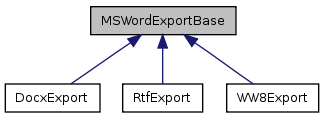
\includegraphics[width=200px,keepaspectratio]{pic/uml.png}
\end{figure}
\begin{figure}[H]
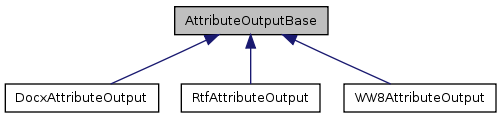
\includegraphics[width=200px,keepaspectratio]{pic/uml-iface.png}
\end{figure}
\begin{itemize}
\item MSWordExportBase: tries to map Writer concepts to MSO
\item AttributeOutputBase: 120+ methods for different resources
\end{itemize}
\end{frame}

\begin{frame}
\frametitle{RTF Export Development}
\framesubtitle{Other new classes}
\begin{itemize}
\item RtfExportFilter: glue between RtfExport and UNO
\item RtfImportFilter: glue between the old RTF import and UNO
\item RtfSdrExport: handles drawings
\item RtfFilter in writerfilter: calls RtfExportFilter and RtfImportFilter via
UNO
\end{itemize}
\end{frame}

\begin{frame}[fragile]
\frametitle{RTF Export Development}
\framesubtitle{Is the goal reached?}
\begin{itemize}
\item No regressions compared to the old filter: mostly
\begin{itemize}
\item still needs more testing, but it's enabled by default
\end{itemize}
\item Smaller code:
\begin{verbatim}
47 files changed
7567 insertions(+), 6981 deletions(-)
\end{verbatim}
More code - due to better structured code, new features.
\item More features: far from lossless conversion, but a number of new features
\end{itemize}
\end{frame}

\begin{frame}
\frametitle{RTF Export Development}
\framesubtitle{Problems}
\begin{itemize}
\item German comments
\item No test files for the old filter
\item Can't wait for the moment when split build will be recommended for development
\item Non-intuitive API's
\end{itemize}
\end{frame}

\begin{frame}[fragile]
\frametitle{RTF Export Development}
\framesubtitle{Hard to remember API's}
\begin{itemize}
\item To send over an SvStream through UNO: \\
\texttt{utl::OStreamWrapper()} to wrap it,
\texttt{utl::UcbStreamHelper::CreateStream()} to unwrap
\item No common base for header / footer - duplicated IsActive() method:
\begin{verbatim}
class SW_DLLPUBLIC SwFmtHeader: public
    SfxPoolItem, public SwClient {...}
class SW_DLLPUBLIC SwFmtFooter: public
    SfxPoolItem, public SwClient {...}
\end{verbatim}
\item Getting the streams from a media descriptor:
\begin{itemize}
\item \texttt{MediaDescriptor::PROP\_STREAMFOROUTPUT()} - output
\item \texttt{MediaDescriptor::PROP\_INPUTSTREAM()} - input
\end{itemize}
\end{itemize}
\end{frame}

\begin{frame}
\frametitle{RTF Export Development}
\framesubtitle{Additional tools}
\begin{itemize}
\item fromhex.py - reads a hexdump from RTF and writes it as a binary
\item prettyprint.py - pretty-prints an RTF file
\item oodocdiff.sh - to test
\begin{itemize}
\item sadly it's mostly useless due to character kerning and other changes
\end{itemize}
\end{itemize}
\end{frame}

\begin{frame}
\frametitle{RTF Export Development}
\framesubtitle{Testing}
\begin{itemize}
\item Cloned ooo-test-files from Cedric / Kohei
\item Added 25 test ODT files
\item Tested with headless writer + jodconverter using UNO
\begin{itemize}
\item that can be now replaced with the batch conversion patches
\end{itemize}
\end{itemize}
\end{frame}

\begin{frame}
\frametitle{RTF Export Development}
\framesubtitle{Documentation}
\begin{itemize}
\item Chicken and egg problem: pointless to read specs from start to end, but
how to just use it as a reference?
\item Necessary resources:
\begin{itemize}
\item Rich Text Format (RTF) Specification, version 1.9.1 (Word 2007)
\item Object Linking and Embedding (OLE) Data Structures
\item ISO/IEC 29500-1:2008 - OOXML spec
\item Word Binary File Format (.doc) Structure Specification
\end{itemize}
\end{itemize}
\end{frame}

\begin{frame}
\frametitle{RTF Export Development}
\framesubtitle{Bookmarks}
Before:
\begin{figure}[H]
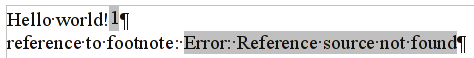
\includegraphics[width=200px,keepaspectratio]{pic/bookmark-old.png}
\end{figure}
After:
\begin{figure}[H]
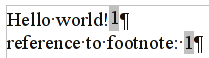
\includegraphics[width=100px,keepaspectratio]{pic/bookmark-new.png}
\end{figure}
\end{frame}

\begin{frame}
\frametitle{RTF Export Development}
\framesubtitle{Character properties}
Before:
\begin{figure}[H]
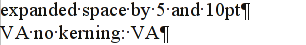
\includegraphics[width=150px,keepaspectratio]{pic/charprops-old.png}
\end{figure}
After:
\begin{figure}[H]
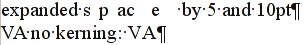
\includegraphics[width=150px,keepaspectratio]{pic/charprops-new.png}
\end{figure}
\end{frame}

\begin{frame}
\frametitle{RTF Export Development}
\framesubtitle{Charts (and other OLE objects)}
Before:
\begin{figure}[H]

\includegraphics[width=120px,keepaspectratio]{pic/chart-old.png}
\end{figure}
After:
\begin{figure}[H]
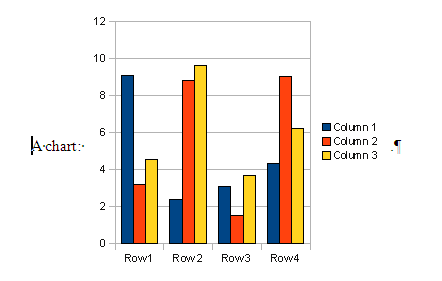
\includegraphics[width=120px,keepaspectratio]{pic/chart-new.png}
\end{figure}
\end{frame}

\begin{frame}
\frametitle{RTF Export Development}
\framesubtitle{Drawings}
Before:
\begin{figure}[H]
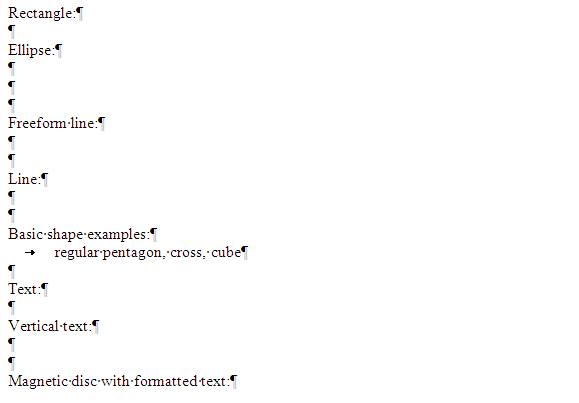
\includegraphics[width=120px,keepaspectratio]{pic/draw-old.png}
\end{figure}
After:
\begin{figure}[H]
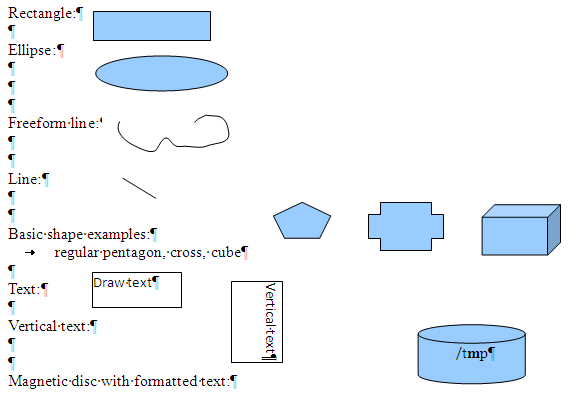
\includegraphics[width=120px,keepaspectratio]{pic/draw-new.png}
\end{figure}
\end{frame}

\begin{frame}
\frametitle{RTF Export Development}
\framesubtitle{Forms}
Before:
\begin{figure}[H]

\includegraphics[width=150px,keepaspectratio]{pic/forms-old.png}
\end{figure}
After:
\begin{figure}[H]
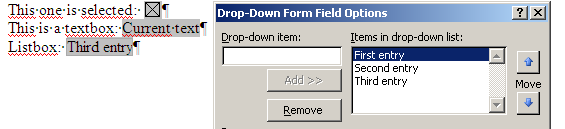
\includegraphics[width=150px,keepaspectratio]{pic/forms-new.png}
\end{figure}
\end{frame}

\begin{frame}
\frametitle{RTF Export Development}
\framesubtitle{Line numbering}
Before:
\begin{figure}[H]
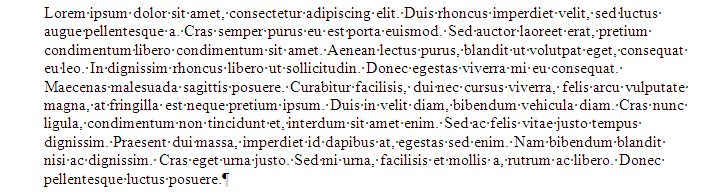
\includegraphics[width=200px,keepaspectratio]{pic/linenum-old.png}
\end{figure}
After:
\begin{figure}[H]
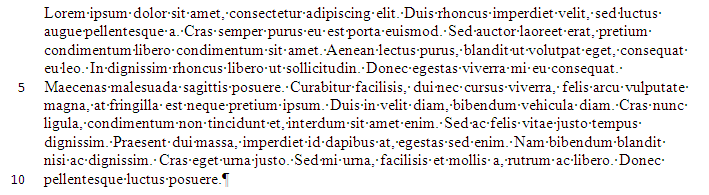
\includegraphics[width=200px,keepaspectratio]{pic/linenum-new.png}
\end{figure}
\end{frame}

\begin{frame}
\frametitle{RTF Export Development}
\framesubtitle{Mathematical Expressions}
Before:
\begin{figure}[H]

\includegraphics[width=100px,keepaspectratio]{pic/math-old.png}
\end{figure}
After:
\begin{figure}[H]
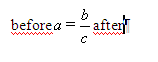
\includegraphics[width=100px,keepaspectratio]{pic/math-new.png}
\end{figure}
\end{frame}

\begin{frame}
\frametitle{RTF Export Development}
\framesubtitle{Editing Mathematical Expressions}
\begin{figure}[H]
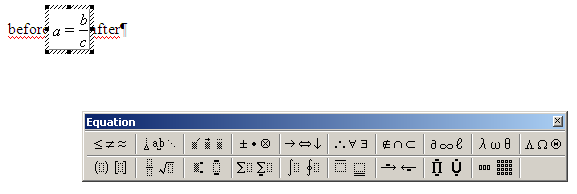
\includegraphics[width=250px,keepaspectratio]{pic/math-new-edit.png}
\end{figure}
\end{frame}

\begin{frame}
\frametitle{RTF Export Development}
\framesubtitle{Special Page Breaks}
Test: normal, right (RTF calls it 'odd'), right again (the last one will be a double break) \\ Before:
\begin{figure}[H]

\includegraphics[width=250px,keepaspectratio]{pic/pagebreak-special-old.png}
\end{figure}
After:
\begin{figure}[H]

\includegraphics[width=250px,keepaspectratio]{pic/pagebreak-special-new.png}
\end{figure}
\end{frame}

\begin{frame}
\frametitle{RTF Export Development}
\framesubtitle{Page Numbering}
Before:
\begin{figure}[H]
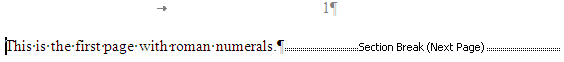
\includegraphics[width=250px,keepaspectratio]{pic/pagenum-restart-old1.png}
\end{figure}
\begin{figure}[H]
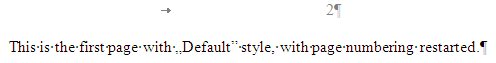
\includegraphics[width=200px,keepaspectratio]{pic/pagenum-restart-old2.png}
\end{figure}
After:
\begin{figure}[H]
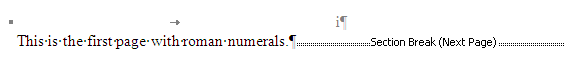
\includegraphics[width=250px,keepaspectratio]{pic/pagenum-restart-new1.png}
\end{figure}
\begin{figure}[H]
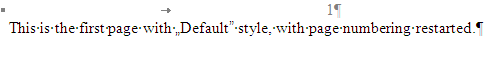
\includegraphics[width=200px,keepaspectratio]{pic/pagenum-restart-new2.png}
\end{figure}
\end{frame}

\begin{frame}
\frametitle{RTF Export Development}
\framesubtitle{Pictures in Wordpad}
Before:
\begin{figure}[H]
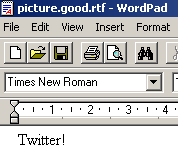
\includegraphics[width=75px,keepaspectratio]{pic/picture-wp-old.png}
\end{figure}
After:
\begin{figure}[H]
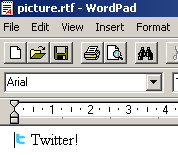
\includegraphics[width=75px,keepaspectratio]{pic/picture-wp-new.png}
\end{figure}
\end{frame}

\begin{frame}
\frametitle{RTF Export Development}
\framesubtitle{Post-it Field}
Before:
\begin{figure}[H]

\includegraphics[width=250px,keepaspectratio]{pic/postit-old.png}
\end{figure}
After:
\begin{figure}[H]
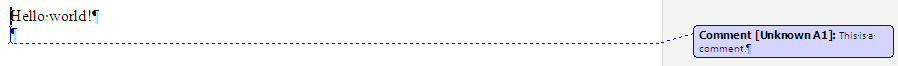
\includegraphics[width=250px,keepaspectratio]{pic/postit-new.png}
\end{figure}
\end{frame}

\begin{frame}
\frametitle{RTF Export Development}
\framesubtitle{Sections: Column Break}
Before:
\begin{figure}[H]
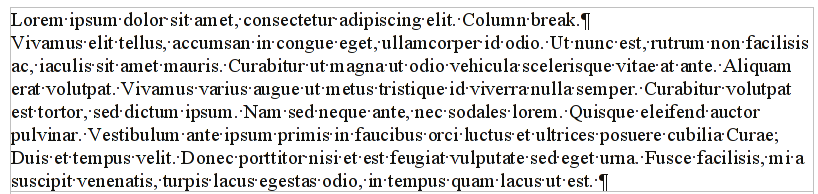
\includegraphics[width=250px,keepaspectratio]{pic/section-column-break-old.png}
\end{figure}
After:
\begin{figure}[H]
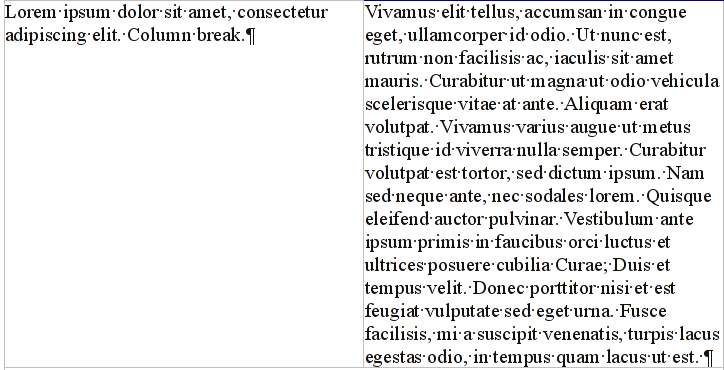
\includegraphics[width=200px,keepaspectratio]{pic/section-column-break-new.png}
\end{figure}
\end{frame}

\begin{frame}
\frametitle{RTF Export Development}
\framesubtitle{Protected Sections}
Before:
\begin{figure}[H]
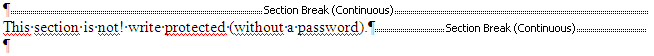
\includegraphics[width=250px,keepaspectratio]{pic/sections-readonly-old.png}
\end{figure}
After:
\begin{figure}[H]
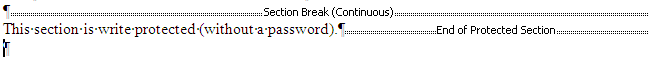
\includegraphics[width=250px,keepaspectratio]{pic/sections-readonly-new.png}
\end{figure}
\end{frame}

\begin{frame}
\frametitle{RTF Export Development}
\framesubtitle{Nested Tables}
Before:
\begin{figure}[H]
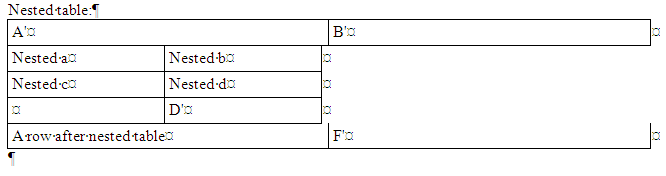
\includegraphics[width=250px,keepaspectratio]{pic/table-nested-old.png}
\end{figure}
After:
\begin{figure}[H]
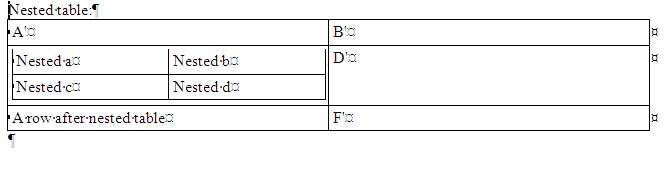
\includegraphics[width=250px,keepaspectratio]{pic/table-nested-new.png}
\end{figure}
\end{frame}

\begin{frame}
\frametitle{RTF Export Development}
\framesubtitle{Table of Contents}
Before:
\begin{figure}[H]
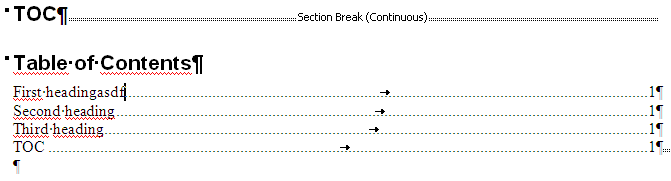
\includegraphics[width=250px,keepaspectratio]{pic/toc-old.png}
\end{figure}
After:
\begin{figure}[H]
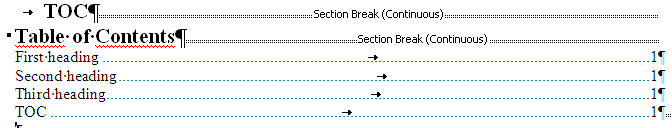
\includegraphics[width=250px,keepaspectratio]{pic/toc-new.png}
\end{figure}
\end{frame}

\begin{frame}
\frametitle{Acknowledgements}
In no particular order:
\begin{itemize}
\item Cedric and Kendy: my mentors
\item Thorsten: testing ideas
\item Kohei: when hacking in the night
\item Bubli: when the Czech guys were not on IRC
\item Petr: patching issues
\item everyone else who helped on \texttt{\#go-oo}
\end{itemize}
\end{frame}

\begin{frame}
\frametitle{References}
\begin{itemize}
\item LibreOffice: \url{http://www.documentfoundation.org/develop/}
\item SoC: \url{http://code.google.com/soc/}
\item New RTF export filter: \url{http://cgit.freedesktop.org/~vmiklos/ooo-gsoc/}
\end{itemize}
\end{frame}

\end{document}
